\chapter{Methodology}

\section{Datasets}

\subsubsection{Offline (PromptReco)}
\begin{itemize}
    \item pp collisions (Separately study 2016 and 2018 data)
    \item 4 different primary datasets: ZeroBias, JetHT, EGamma, SingleMuon
    \item Each lumisection (datapoint) contains
    \begin{itemize}
        \item Selected $n$ histograms of physics quantity e.g. JetPt, JetEta, JetPhi, etc.
        \item Represent one histogram with 7 numbers
        \item $n \times 7$ Features
    \end{itemize}
    \item Good LS defined in Golden JSON else Bad LS
\end{itemize}

\subsection{Histogram Representation}
\begin{figure}[h!]
    \centering
    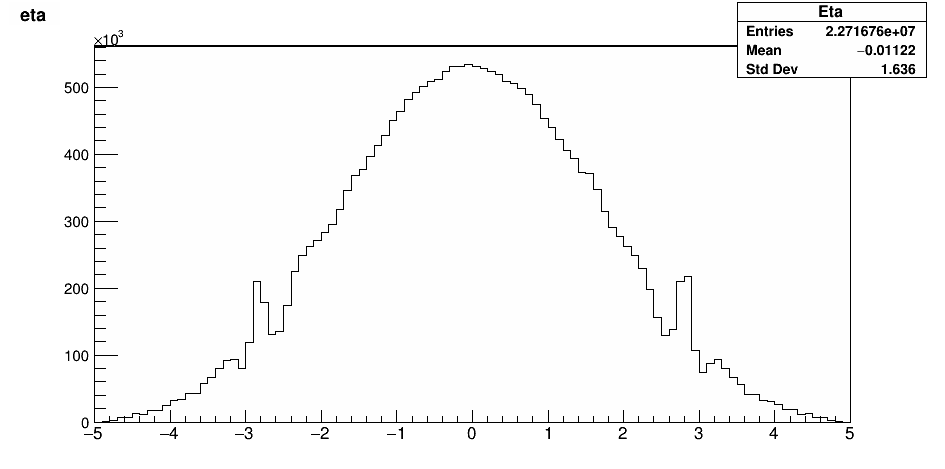
\includegraphics[width=0.7\textwidth]{images/ex_eta_dist.png}
    \caption{$\eta$ distribution, Image taken from DQM GUI}
    \label{fig:ex_eta_dist}
\end{figure}

In order to mimic the offline shifter that looking at the histogram and certify data by that.
Then we decided represent a single histogram with seven quantities instead of feeding all of those to the model because it would be an overwhelming large features.
The explicit example is to consider one histogram as Figure \ref{fig:ex_eta_dist}

Here are the simple step for picking up our represented vector
\begin{itemize}
    \item Quantize [10\%, 30\%, 50\%, 70\%, 90\%] of the histogram (For 2016 data, we quantize [0\%, 25\%, 50\%, 75\%, 100\%] of the histogram)
    \item Combine mean and rms
    \item Use these 7 values to represent one histogram
\end{itemize}


\subsection{Data Preprocessing}

For numerically convenient, we transform the each data point by using 

\textbf{MinMaxScalar Transformation} The mathematical expression are represented by consider lumisection $i$ and features $j$

\begin{equation}
    x_{ij}' \leftarrow \frac{x_{ij} - \min_{\forall i\in S_{\text{train}}}\{x_{ij}\}}{\max_{\forall i\in S_{\text{train}}}\{x_{ij}\} - \min_{\forall i\in S_{\text{train}}}\{x_{ij}\} }
\end{equation}
In principle, each feature in our data should be in range zero to unity.

\section{Semi-Supervised Learning}
We exploiding a various unsupervised model from a beautiful simple one to more complicate neural network which are
\begin{itemize}
    \item Sch\"{o}lkopf's One-Class SVM
    \item Isolation Forest
    \item 4 Flavours of Autoencoder
\end{itemize}
For training the model by feeding only good LS as well as validate it with good LS to ensure the learning curve is the appropriate for hyper-parameters configurations.
After the training process is done, we test it with both good and bad LS. Consequently, it's falling into \textbf{Semi-supervised Learning} category.

\subsection{Sch\"{o}lkopf's One-Class SVM}
Support vector machine (SVM) is one of the most popular machine learning model since it has no randomness and beautiful straightforward way to express.
There is a way to tweak the original one to interpret as the radious-like hyperplane where the inlier of data are feeding and mapped to more than one radius with a soft margin controlled by factor $\nu$ as interpret in \cite{oneclasssvm}.
By minimizing
\begin{equation}
\frac{||w||^2}{2} + \frac{1}{\nu l}\sum_{i=1}^l \xi_i - \rho
\end{equation}
Subject to
\begin{equation}
    w \cdot \Phi(x_i) \geqslant \rho - \xi_i \ ,\ \xi_i \geqslant 0
\end{equation}
With Gaussian Base Radial function (GBF) as a kernel like equation \ref{eq:gbf}
\begin{equation}\label{eq:gbf}
    k(\mathbf{x}, \mathbf{y}) = \exp(-\gamma||\mathbf{x} - \mathbf{y}||^2)
\end{equation}

\subsection{Isolation Forest}
The idea of bagging the sample and construct a tree are incredibly beautiful are interpreted and adapt in a way that unsupervised learning are come to the place are study by \cite{isolation_forest}.
Forest are construct by picking up subsampling ($\Psi$) and Iteratively picking up features and random value to construct the node (equivalent to step function), then Anomaly score evaluate from average depth of the instance over forest
\begin{equation}
    s(x, \Psi) = \exp^{-<h(x)>/c(\Psi)}
\end{equation} 
where
\begin{itemize}
    \item $h(x)$ is the depth in tree $h$
    \item $c(\Psi)$ normalization factor growing as $\log_2(\Psi)$ from branching
\end{itemize}

\subsection{Autoencoder (AE)}
Let start with the hyper-parameters and configurations of our model
\subsubsection*{Truncated normal initializer}
For model weight initializer, we are using truncated normal initializer which basically you take a gaussian distribution and putting the cutoff only inside $\pm2\sigma$ as in the Figure \ref{fig:normal_dist} to prevent some high absolute value that might leading to divergence of model in the training process.

In our case, we set up $\sigma=1$ and $\mu=1$ 
\begin{figure}[h!]
    \centering
    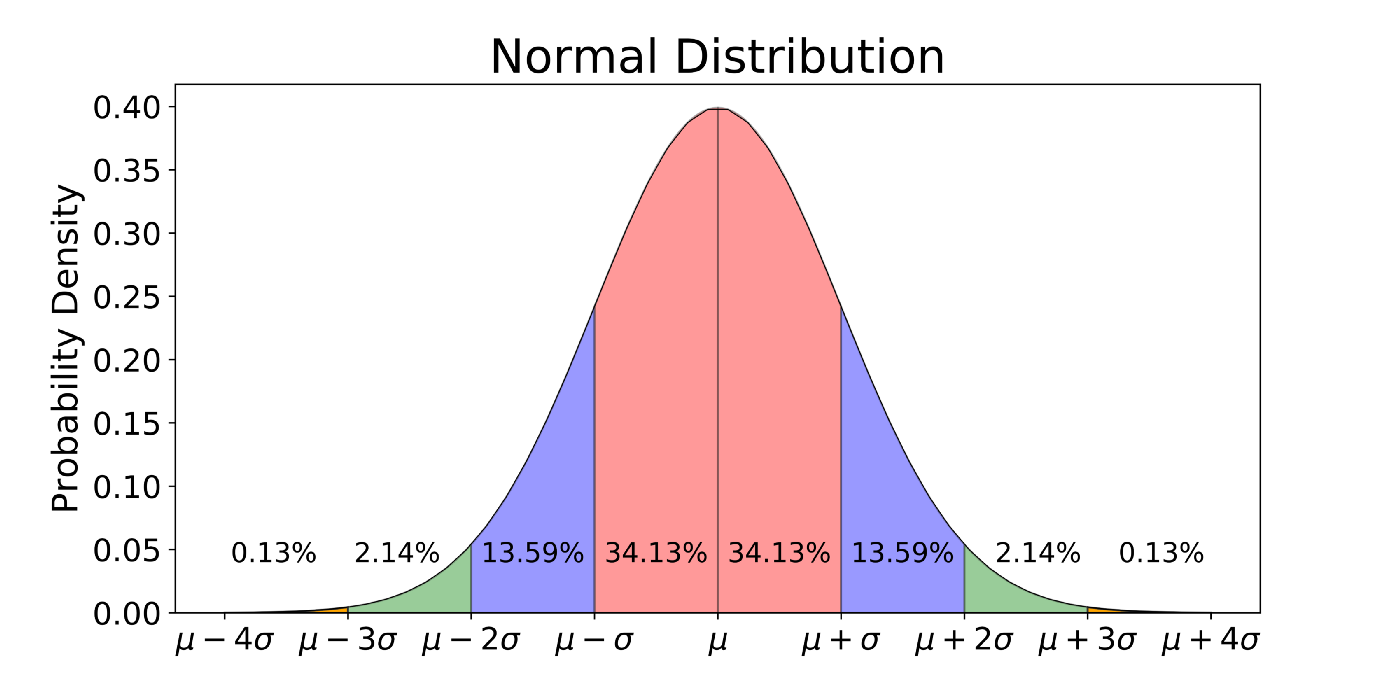
\includegraphics[width=0.7\textwidth]{images/normal_dist.png}
    \caption{Gaussian distribution, retrieved from https://towardsdatascience.com/understanding-the-68-95-99-7-rule-for-a-normal-distribution-b7b7cbf760c2}
    \label{fig:normal_dist}
\end{figure}

\subsubsection*{Adam Optimizer}
Adam stands for \textbf{adaptive moment estimation} \cite{adam}. Basically, it's combine Momentum optimization and RMSProp to keep the residue of the gradients decaying from the previous update.
We set up $lr = 10^{-4}$ (learning rate), $\beta_1 = 0.7$ and $\beta_2$ = 0.9.
\vspace{0.4in}
\par There are 4 flavours of our autoencoder that we constructed

\subsubsection{Vanilla AE}
\begin{figure}[h!]
    \centering
    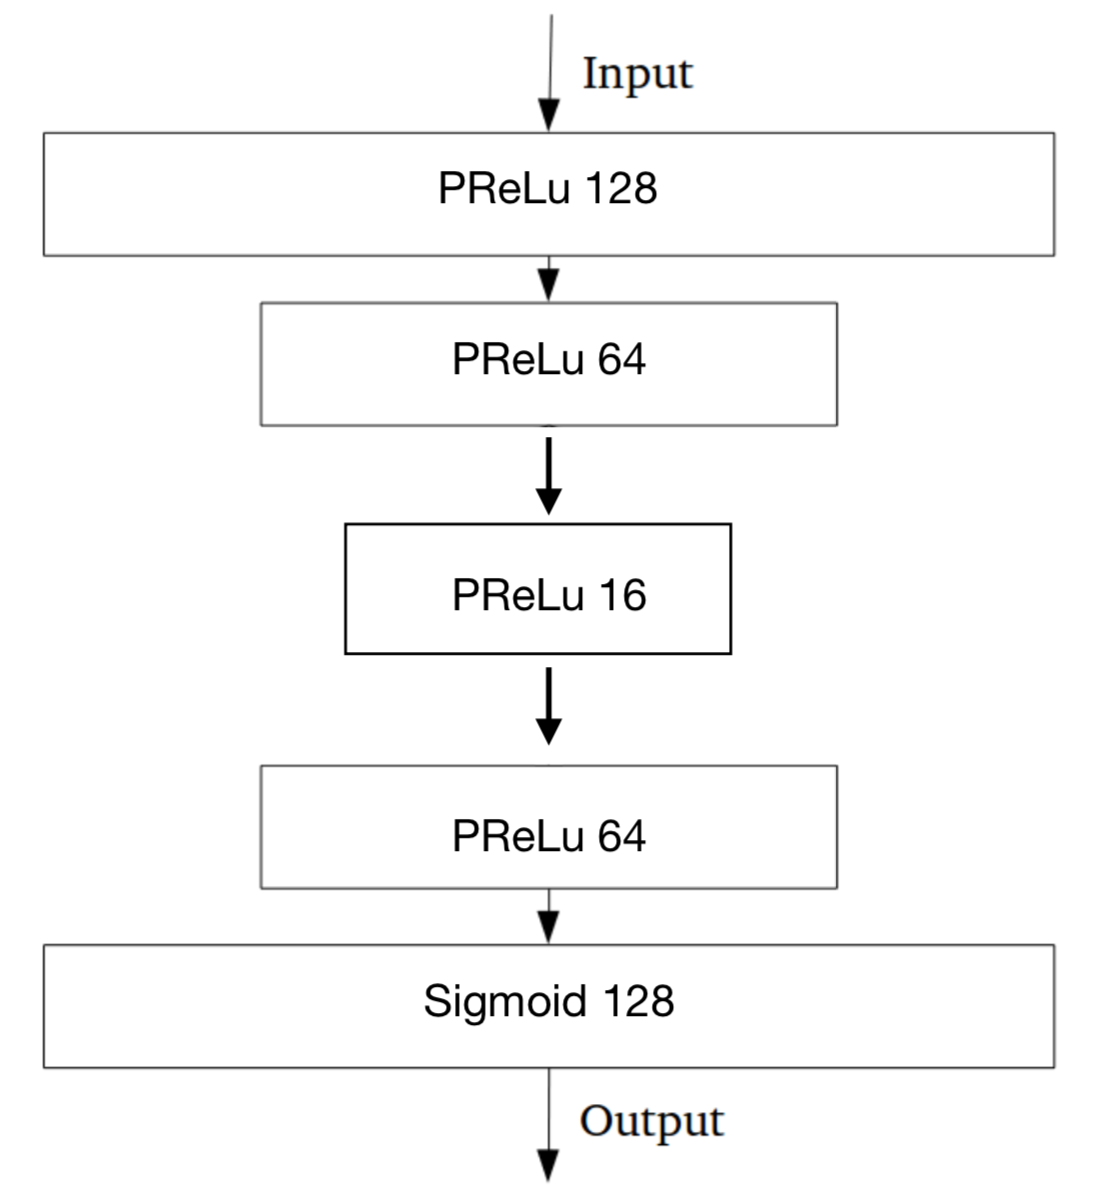
\includegraphics[width=0.4\textwidth]{images/vanilla_ae.png}
    \caption{Body of Vanilla AE}
    \label{fig:vanilla_ae}
\end{figure}
\begin{itemize}
    \item Concise the information into small latent space and reconstruct
    \item Loss function is designed by taking the square different reconstructed vector from the latent space and origin vector as equation \ref{eq:loss_vanilla}
\end{itemize}
\begin{equation}\label{eq:loss_vanilla}
    \mathcal{L}_{\text{tot}} \equiv \frac{1}{N}\sum_i^N |x_i-\tilde{x}_i|^2
\end{equation}

\subsubsection{Sparse AE}
\begin{itemize}
    \item Similar to Vanilla AE
    \item Tweak by \textcolor[RGB]{255,69,0}{L1 Regularizaion (Prevent overfitting)}
    \item Loss function
    \begin{equation}
        \mathcal{L}_{\text{tot}} \equiv \frac{1}{N}\sum_i^N |x_i-\tilde{x}_i|^2 + \textcolor[RGB]{255,69,0}{\lambda_{\text{s}}\sum_j||w_j||}
    \end{equation}
    \item where $\lambda_{\text{s}} = 10^{-5}$
\end{itemize}

\subsubsection{Contractive AE}
\begin{itemize}
    \item Definition
    \begin{equation}
        \textcolor[RGB]{0,128,0}{||J_h(x)||^2 \equiv \frac{1}{N}\sum_{ij}\left(\frac{\partial h_j}{\partial x_i}\right)^2}
    \end{equation}
    \item where $h_j$ is activation function
    \item In our cases
    \begin{itemize}
        \item PReLu activation function
        \begin{equation}
            ||J_h(x)||^2 = \frac{1}{N}\sum_i^N\sum_j[\alpha_j H(-(w_{jk}x^{ik}+b_j)) + H(w_{jk}x^{ik}+b_j)]\sum_k(w_{jk})^2
        \end{equation}
        \item Sigmoid activation function
        \begin{equation}
            ||J_h(x)||^2 = \frac{1}{N}\sum_{ij}[h_{ij}(1-h_{ij})]\sum_k(w_{jk})^2
        \end{equation}
    \end{itemize}
\end{itemize}

\subsubsection{Variational AE}
\begin{figure}[h!]
    \centering
    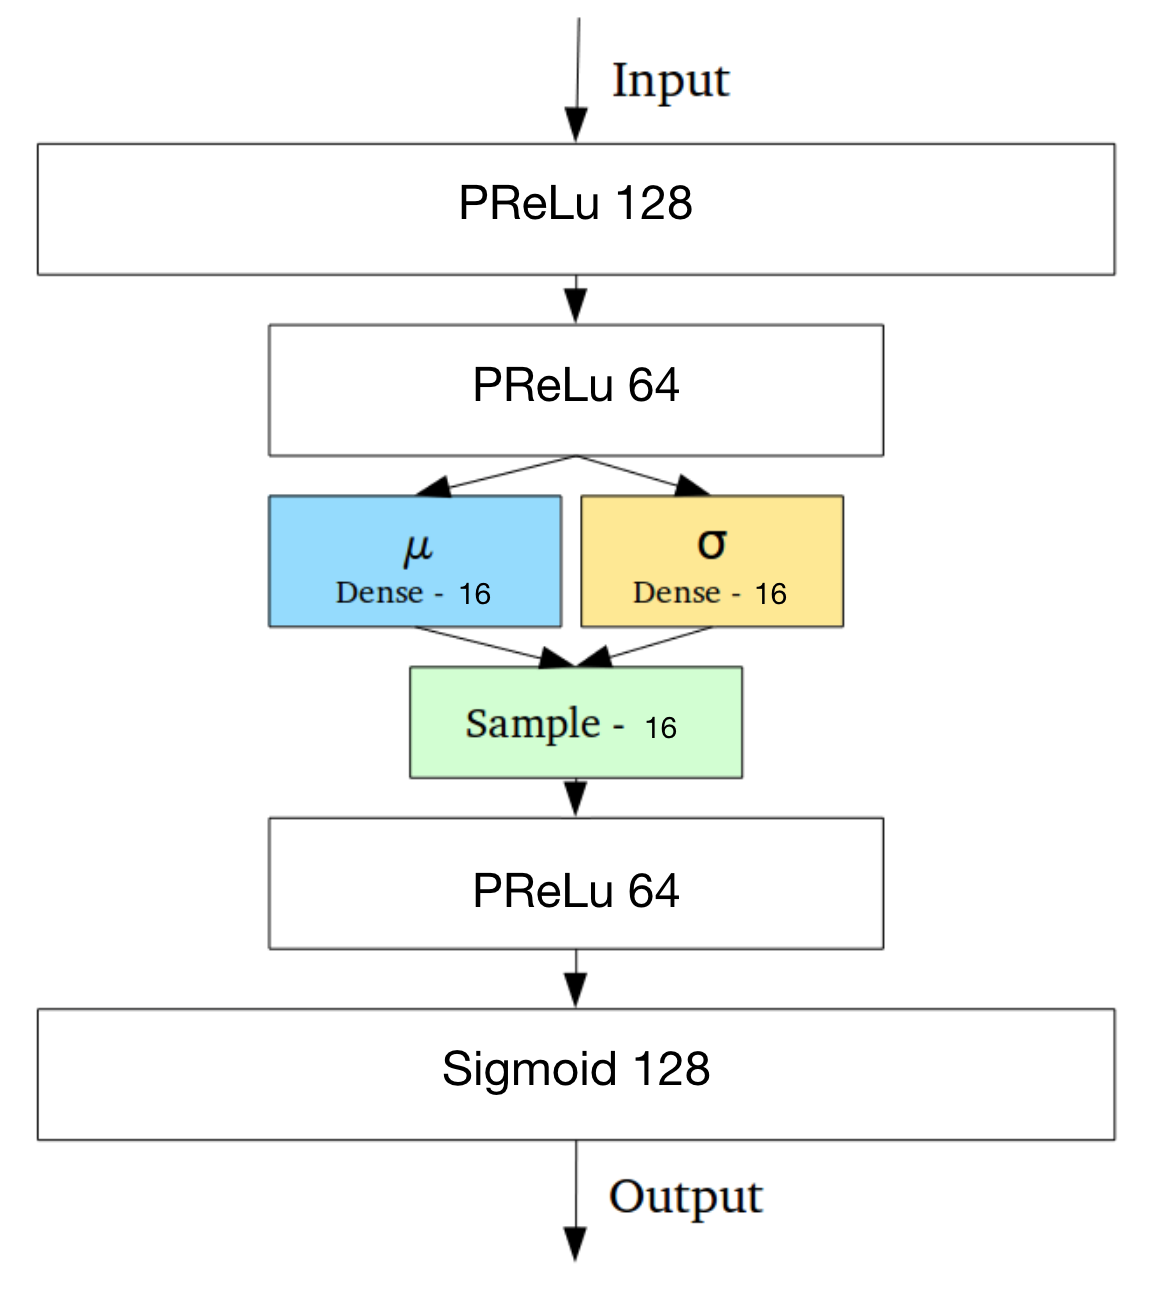
\includegraphics[width=0.4\textwidth]{images/variational_ae.png}
    \caption{Body of Variational AE retrieved from https://towardsdatascience.com/intuitively-understanding-variational-autoencoders-1bfe67eb5daf}
    \label{fig:variational_ae}
\end{figure}

\begin{itemize}
    \item Random \say{new sampling} in latent space by gaussian random generator
    \begin{equation}
        \mathcal{Z} \equiv \mathcal{N}(\mu_i, \sigma_i)
    \end{equation}
    \item Tweak by \textcolor[RGB]{148,0,211}{reduce discontinuity in latent space}
    \item Loss function
    \begin{equation}
        \mathcal{L}_{\text{tot}} = \frac{1}{N}\sum_i^N |x_i-\tilde{x}_i|^2 + \frac{1}{2N}\sum_i^N\sum_k^{n_{\text{latent}}}(\mu_{ik}^2 +\sigma_{ik}^2 - 2\log\sigma_{ik} - 1)
    \end{equation}
\end{itemize}